\documentclass[12pt]{article}
\usepackage[margin=1in]{geometry}
\usepackage{graphicx}
\usepackage{caption}
\usepackage{float}
\usepackage{setspace}
\usepackage{booktabs}
\usepackage{siunitx}
\usepackage{amsmath, amssymb}
\usepackage{hyperref}
\hypersetup{colorlinks=true,linkcolor=blue,urlcolor=blue,citecolor=blue}
\sisetup{per-mode=symbol,detect-all=true}
\onehalfspacing
\title{A Computational Analysis of a Set Parameter Beta-Type Stirling Engine\\and Flywheel Design Optimization}
\author{Thomas Ritten \and Sebastian Hondl \and Peyton Lettau}
\date{Group 29 -- ME4051 -- 9/20/25}
\begin{document}
\maketitle
\section*{Executive Summary}
This report presents a comprehensive computational analysis of a Beta-type Stirling engine with integrated flywheel design optimization. The analysis employs Schmidt thermodynamic modeling, slider-crank kinematics, and three-stage phase optimization to evaluate engine performance and design requirements. Key findings include a cycle efficiency of 24.2\% compared to ideal conditions, optimal phase shift of 103.6° (13.6° above conventional 90°), and successful flywheel design achieving the target coefficient of fluctuation of 0.003. The systematic methodology provides a foundation for parametric studies and design optimization of Stirling engines, while highlighting the significant performance gaps between idealized assumptions and practical implementation.

\section{Introduction}
Beta-type Stirling engines represent a promising technology for waste heat recovery and distributed power generation. This analysis evaluates the complete thermodynamic and dynamic behavior of a specified engine configuration, examining work generation, torque characteristics, speed regulation, and phase optimization. The study employs systematic computational methods to assess both ideal and actual performance, providing insights into design optimization and practical implementation challenges.

\section{System Specifications}
The analysis is based on the following engine and operating parameters:
\begin{table}[H]
  \centering
  \caption{Initial engine and operating parameters (given).}
  \label{tab:params}
  \begin{tabular}{@{}llll@{}}
    \toprule
    \textbf{Parameter} & \textbf{Symbol} & \textbf{Value} & \textbf{Units} \\
    \midrule
    Power piston crank length & $r_{p}$ & \num{0.025} & \si{\meter} \\
    Power piston connecting rod & $\ell_{p}$ & \num{0.075} & \si{\meter} \\
    Displacer crank length & $r_{d}$ & \num{0.02} & \si{\meter} \\
    Displacer connecting rod & $\ell_{d}$ & \num{0.14} & \si{\meter} \\
    Displacer volume & $V_{d}$ & \num{4.0e-5} & \si{\meter\cubed} \\
    Cylinder bore diameter & $D$ & \num{0.05} & \si{\meter} \\
    Phase shift & $\phi$ & $\pi/2$ & \si{\radian} \\
    Compression ratio & $\mathrm{CR}$ & \num{1.7} & --- \\
    Hot temperature & $T_{h}$ & \num{900} & \si{\kelvin} \\
    Cold temperature & $T_{c}$ & \num{300} & \si{\kelvin} \\
    Gas pressure at BDC & $P_{\mathrm{BDC}}$ & \num{500} & \si{\kilo\pascal} (abs) \\
    Atmospheric pressure & $P_{\mathrm{atm}}$ & \num{101.3} & \si{\kilo\pascal} (abs) \\
    Regenerator dead volume & $V_{\mathrm{reg}}$ & \num{2.0e-5} & \si{\meter\cubed} \\
    Flywheel width & $w$ & \num{0.025} & \si{\meter} \\
    Flywheel rim thickness & $t$ & \num{0.05} & \si{\meter} \\
    Flywheel material density & $\rho$ & \num{8000} & \si{\kilo\gram\per\meter\cubed} \\
    Coefficient of fluctuation & $C_{f}$ & \num{0.003} & --- \\
    Average rotational speed & $\overline{\Omega}$ & \num{650} & \si{rpm} \\
    \bottomrule
  \end{tabular}
\end{table}

% (Section removed to meet 10-page limit; not required by deliverables.)
\section{Analysis Methodology}
The computational analysis follows a systematic seven-step approach, beginning with geometric parameter derivation and progressing through kinematic analysis, thermodynamic modeling, torque calculation, flywheel sizing, dynamic simulation, and phase optimization. The crank angle is discretized as \(\theta \in [0,2\pi)\) with 360 evenly spaced points, and the cross-sectional area is \(A = \pi D^{2}/4\).

\subsection{Step 1: Geometric Parameter Derivation}
Initial calculations establish the complete engine geometry from given parameters. The displacer height is calculated as \(h_d = V_d/A\), and power piston positions at BDC and TDC are determined using slider-crank equations to obtain the swept volume \(V_{\text{swept}} = A(x_{\text{TDC}} - x_{\text{BDC}})\). The total cylinder volume at BDC is calculated using the compression ratio: \(V_{\text{total,BDC}} = V_r - V_d + \mathrm{CR} \cdot V_{\text{swept}}/(\mathrm{CR}-1)\). The total cylinder height is then determined as:
\begin{equation}
  H_{\text{tot}} = \frac{V_{\text{total,BDC}}}{A} + h_d + h_{\text{pin}} + \ell_p - r_p,
\end{equation}
where terms account for cold/hot space height, displacer height, pin offset, and connecting rod geometry. The regenerator temperature is set to \(T_r = (T_h + T_c)/2\).

\subsection{Step 2: Slider-Crank Kinematics}
Piston and displacer positions are calculated using slider-crank kinematics with rod obliquity. For crank radius \(r\) and rod length \(\ell\):
\begin{align}
  \beta(\theta) &= \arcsin\!\biggl( \frac{r}{\ell}\,\sin\theta \biggr),\label{eq:beta-def}\\
  x(\theta) &= \ell\,\cos\beta(\theta) - r\,\cos\theta.
\end{align}
This yields \(x_{p}(\theta)\) for the power piston and \(x_{d}(\theta+\phi)\) for the displacer (phase shifted by \(\phi\)).

\subsection{Step 3: Volume Calculations}
Cold and hot space volumes are computed from piston positions. Cold height represents the separation between displacer and power piston; hot height is measured from the space above the displacer:
\begin{align}
  h_{c}(\theta) &= \bigl[x_{d}(\theta+\phi) - x_{p}(\theta)\bigr] - h_{\mathrm{pin}} - \tfrac{1}{2}h_{d},\\
  h_{h}(\theta) &= H_{\mathrm{tot}} - \tfrac{1}{2}h_{d} - x_{d}(\theta+\phi),
\end{align}
The corresponding volumes are:
\begin{align}
  V_{c}(\theta) &= A\,h_{c}(\theta), & V_{h}(\theta) &= A\,h_{h}(\theta), & V_{r} &= \text{const}.
\end{align}

\subsection{Step 4: Schmidt Thermodynamic Analysis}
The total gas mass is determined at bottom dead center (BDC, \(\theta=0\)) using the known absolute pressure \(P_{\mathrm{BDC}}\):
\begin{align}
  m &= \frac{P_{\mathrm{BDC}}}{R}\biggl( \frac{V_{c}(0)}{T_{c}} + \frac{V_{r}}{T_{r}} + \frac{V_{h}(0)}{T_{h}} \biggr).
\end{align}
Instantaneous pressure is calculated using the Schmidt relation:
\begin{align}
  P(\theta) &= \frac{m\,R}{\dfrac{V_{c}(\theta)}{T_{c}} + \dfrac{V_{r}}{T_{r}} + \dfrac{V_{h}(\theta)}{T_{h}} }.
\end{align}
Cycle work is evaluated numerically using trapezoidal integration:
\begin{equation}
  W = \oint P\,\mathrm{d}V \approx \sum_{k} P(\theta_{k})\,\Delta V(\theta_{k}).
\end{equation}

\subsection{Step 5: Torque Calculation}
Pressure is converted to torque through the power piston. The net axial force is \(F_{p}(\theta) = \bigl(P(\theta)-P_{\mathrm{atm}}\bigr)\,A\). Using the rod obliquity angle \(\beta\) from Eq.~\eqref{eq:beta-def} and crank radius \(r_{p}\), the instantaneous torque is:
\begin{equation}
  \tau(\theta) = -\,F_{p}(\theta)\,\frac{r_{p}\,\sin\theta}{\cos\beta(\theta)}.
\end{equation}

\subsection{Step 6: Flywheel Sizing}
The flywheel is sized to achieve the target coefficient of fluctuation. Torque deviation about the mean is calculated as:
\begin{equation}
  T_{\text{dev}}(\theta) = \tau(\theta) - \overline{\tau}, \quad \text{where } \overline{\tau} = \frac{1}{2\pi}\int_0^{2\pi} \tau(\theta)\,\mathrm{d}\theta.
\end{equation}
Energy fluctuation \(\Delta E\) is the peak-to-peak of the integrated torque deviation, yielding the required inertia:
\begin{equation}
  I_{\mathrm{req}} = \frac{\Delta E}{C_{f}\,\omega_{\!\text{avg}}^{2}}.
\end{equation}
The flywheel is modeled as a thick ring with moment of inertia:
\begin{equation}
  I_{\mathrm{rim}}(R) = \tfrac{1}{2}\,M(R)\,\bigl(R^{2}+R_{\mathrm{in}}^{2}\bigr),\quad M(R)=\rho\,\pi w\,\bigl(R^{2}-R_{\mathrm{in}}^{2}\bigr),\quad R_{\mathrm{in}}=R-t.
\end{equation}
A fixed-point iteration solves \(I_{\mathrm{rim}}(R)=I_{\mathrm{req}}\) using the initial guess \(R^{(0)} = \sqrt{I_{\mathrm{req}}/(\pi\,\rho\,w\,t)} + t/2\) and the update rule:
\begin{equation}
  R^{(k+1)} = R^{(k)}\,\eta^{1/3},\qquad \eta = \frac{I_{\mathrm{req}}}{I_{\mathrm{act}}},\qquad R_{\mathrm{in}}=R^{(k+1)}-t.
\end{equation}
Convergence occurs when the relative error drops below tolerance. Final dimensions are \(D_{\mathrm{out}}=2R\), \(D_{\mathrm{in}}=2R_{\mathrm{in}}\), and mass \(M(R)\).

\subsection{Step 7: Dynamic Simulation}
Engine speed variation is simulated using the work-energy theorem. Load torque equals mean engine torque for steady-state operation. The net torque drives angular acceleration, and speed is updated using cumulative work \(W_{\text{net}}(\theta)\):
\begin{equation}
  \Omega^{2}(\theta) = \Omega_{\!\text{avg}}^{2} + \frac{2\,W_{\text{net}}(\theta)}{I},\qquad \Omega(\theta) = \sqrt{\Omega^{2}(\theta)}.
\end{equation}
The speed profile is normalized to maintain the target average while preserving the fluctuation pattern.

\subsection{Step 8: Phase Optimization}
Phase shift optimization employs a three-stage refinement strategy to maximize power output. Stage 1 performs a coarse scan from \(30^{\circ}\) to \(150^{\circ}\) in \(2^{\circ}\) increments. Stage 2 refines within \(\pm6^{\circ}\) of the best candidate at \(0.1^{\circ}\) resolution. Stage 3 pinpoints the optimum within \(\pm0.5^{\circ}\) at \(0.01^{\circ}\) resolution. At each phase, mean torque is integrated over \(\theta\), power is calculated as \(\bar{\tau}\,\omega_{\!\text{avg}}\), and the \(\phi\) maximizing power is selected.

\section{Results and Discussion}
The computational analysis provides comprehensive performance evaluation across all system components. Results are organized following the systematic methodology, progressing from kinematic analysis through thermodynamic performance, dynamic behavior, and optimization outcomes.

\subsection{Kinematic Analysis}
The kinematic analysis establishes the volume envelopes that drive thermodynamic processes. The power piston achieves a 50.00 mm stroke with maximum position at 100.00 mm, while the displacer stroke is 40.00 mm with maximum position at 160.00 mm. Total volume varies from 140.25 to 238.42 cm³, achieving the specified compression ratio of 1.70. Hot and cold volumes range from 32.26–110.80 cm³ and 35.61–163.18 cm³, respectively, with a constant 20.00 cm³ regenerator volume. These volume variations establish the pressure swing that drives cycle work production.

\subsection{Thermodynamic Performance}
The Schmidt analysis reveals significant performance characteristics. Pressure ranges from 474.63 to 1178.83 kPa with a mean of 730.39 kPa and pressure ratio of 2.48. This variation is substantially lower than ideal Stirling cycle predictions due to dead volumes and simplified Schmidt assumptions.

Figure~\ref{fig:pv_diagram} compares the actual engine cycle with the ideal Stirling cycle, providing insight into the thermodynamic performance.

\begin{figure}[htbp]
  \centering
  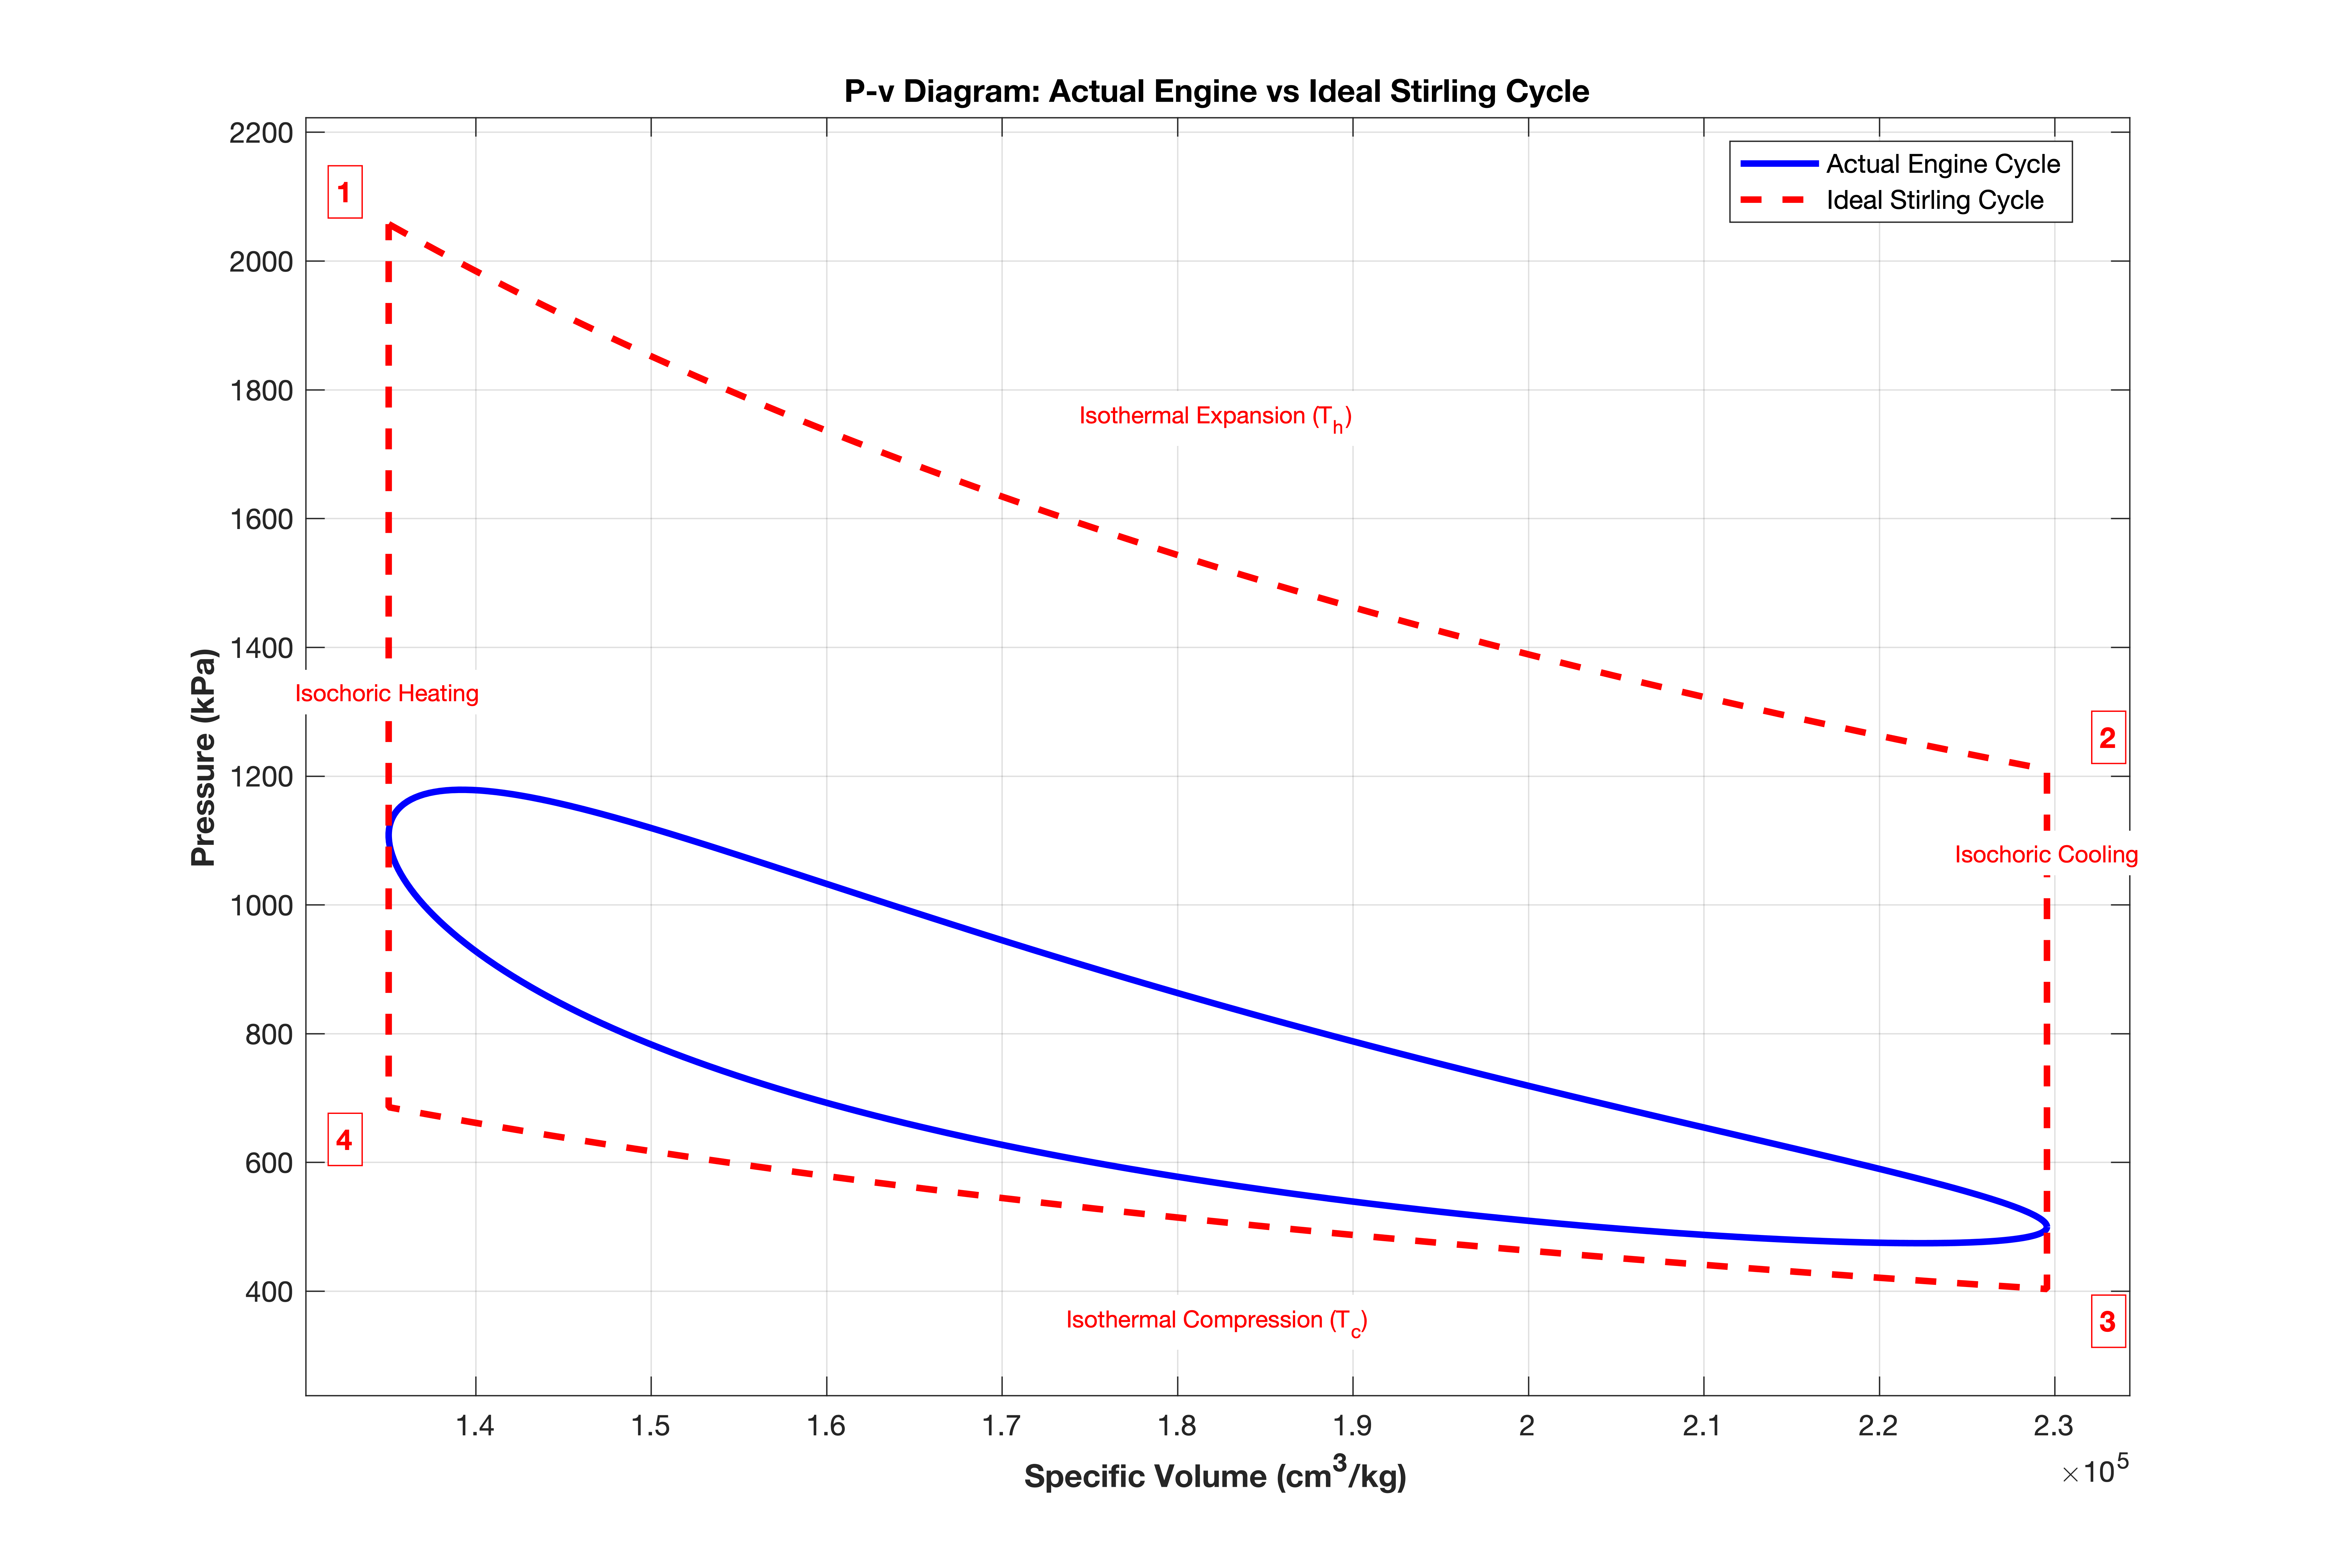
\includegraphics[width=0.8\linewidth]{../pv_diagram.png}
  \caption{P-v diagram comparing the actual engine cycle with the ideal Stirling cycle.}
  \label{fig:pv_diagram}
\vspace{-6pt}\end{figure}

The ideal Stirling cycle produces 94.9 J of work per cycle, while the actual Schmidt analysis yields 23.0 J, resulting in a cycle efficiency of 24.2\%. This substantial performance gap demonstrates the significant impact of dead volumes, non-ideal heat transfer, and simplified thermodynamic assumptions.

\subsection{Torque and Power Analysis}
The torque analysis, shown in Figure~\ref{fig:torque_angle}, demonstrates the engine\textquotesingle s instantaneous power production capability.

\begin{figure}[htbp]
  \centering
  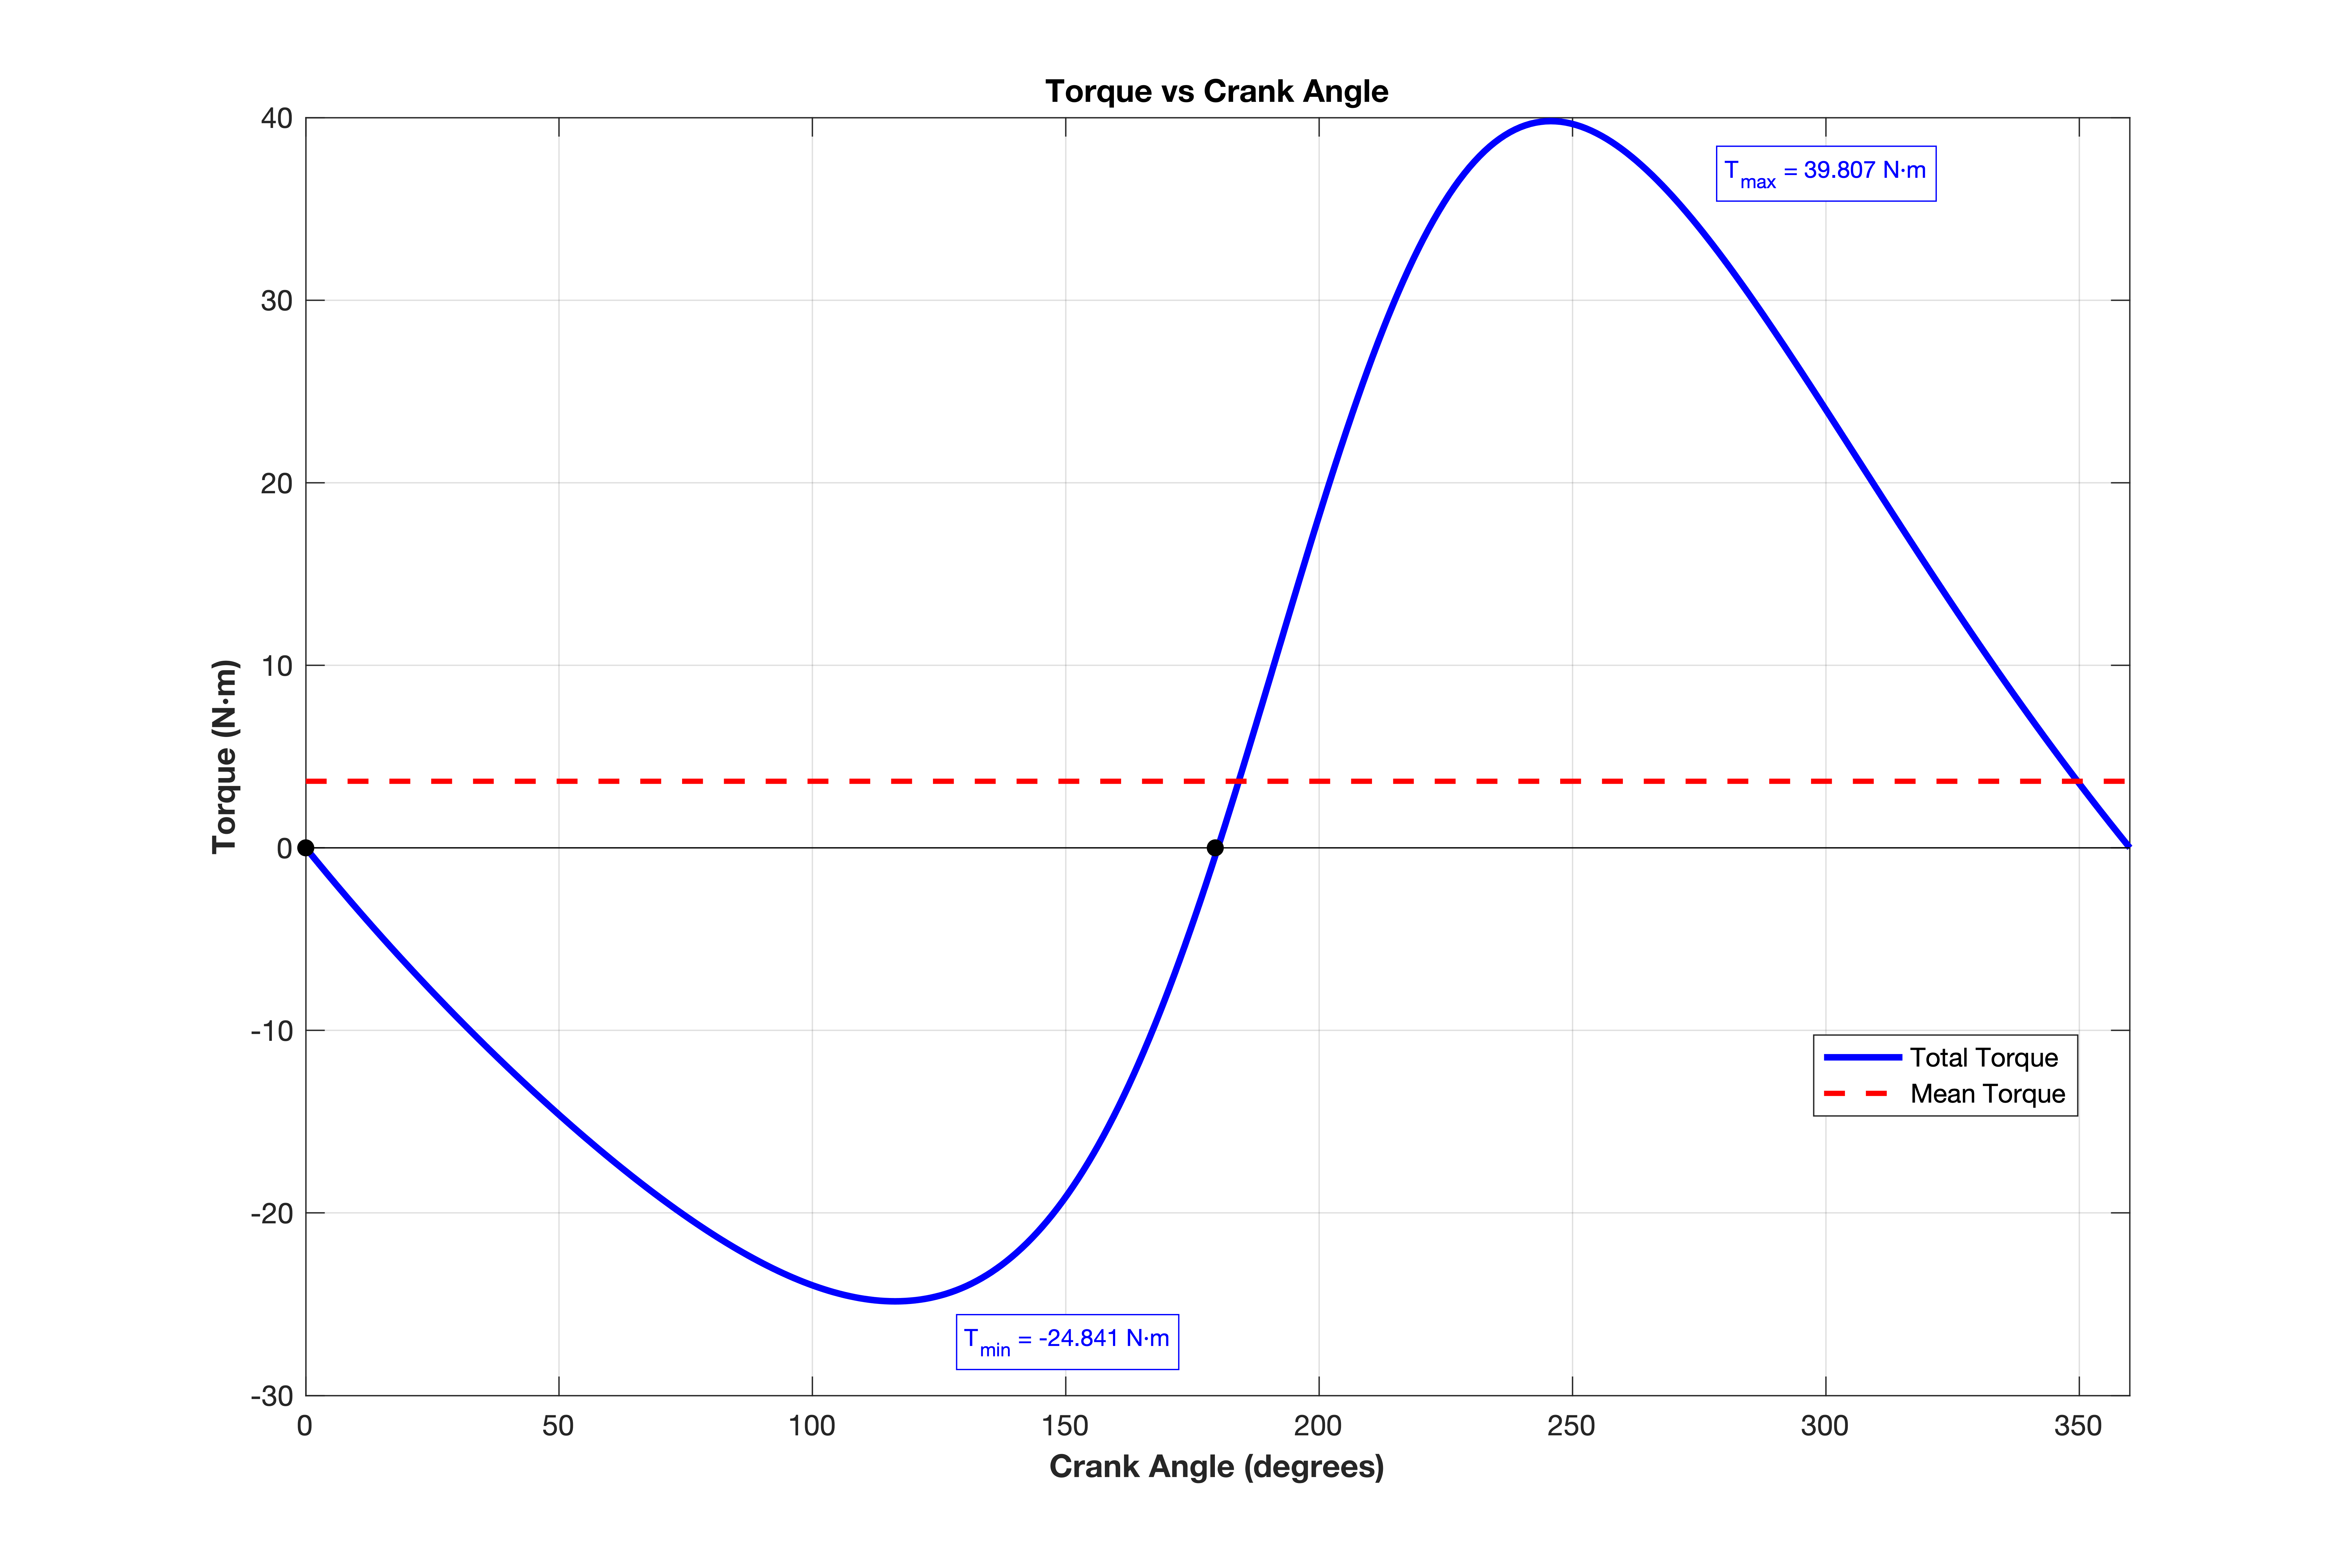
\includegraphics[width=0.8\linewidth]{../torque_vs_angle.png}
  \caption{Torque vs. crank angle showing the instantaneous torque production throughout the cycle.}
  \label{fig:torque_angle}
\vspace{-6pt}\end{figure}

Total torque ranges from -24.841 to 39.807 N·m with a positive mean of 3.648 N·m, confirming net work production capability. The torque variation reflects pressure-volume work interactions, with positive torque during expansion and negative torque during compression phases.

\subsection{Dynamic Performance and Speed Regulation}
The angular velocity analysis, shown in Figure~\ref{fig:angular_velocity}, demonstrates the flywheel\textquotesingle s effectiveness in maintaining consistent rotational speed.

\begin{figure}[htbp]
  \centering
  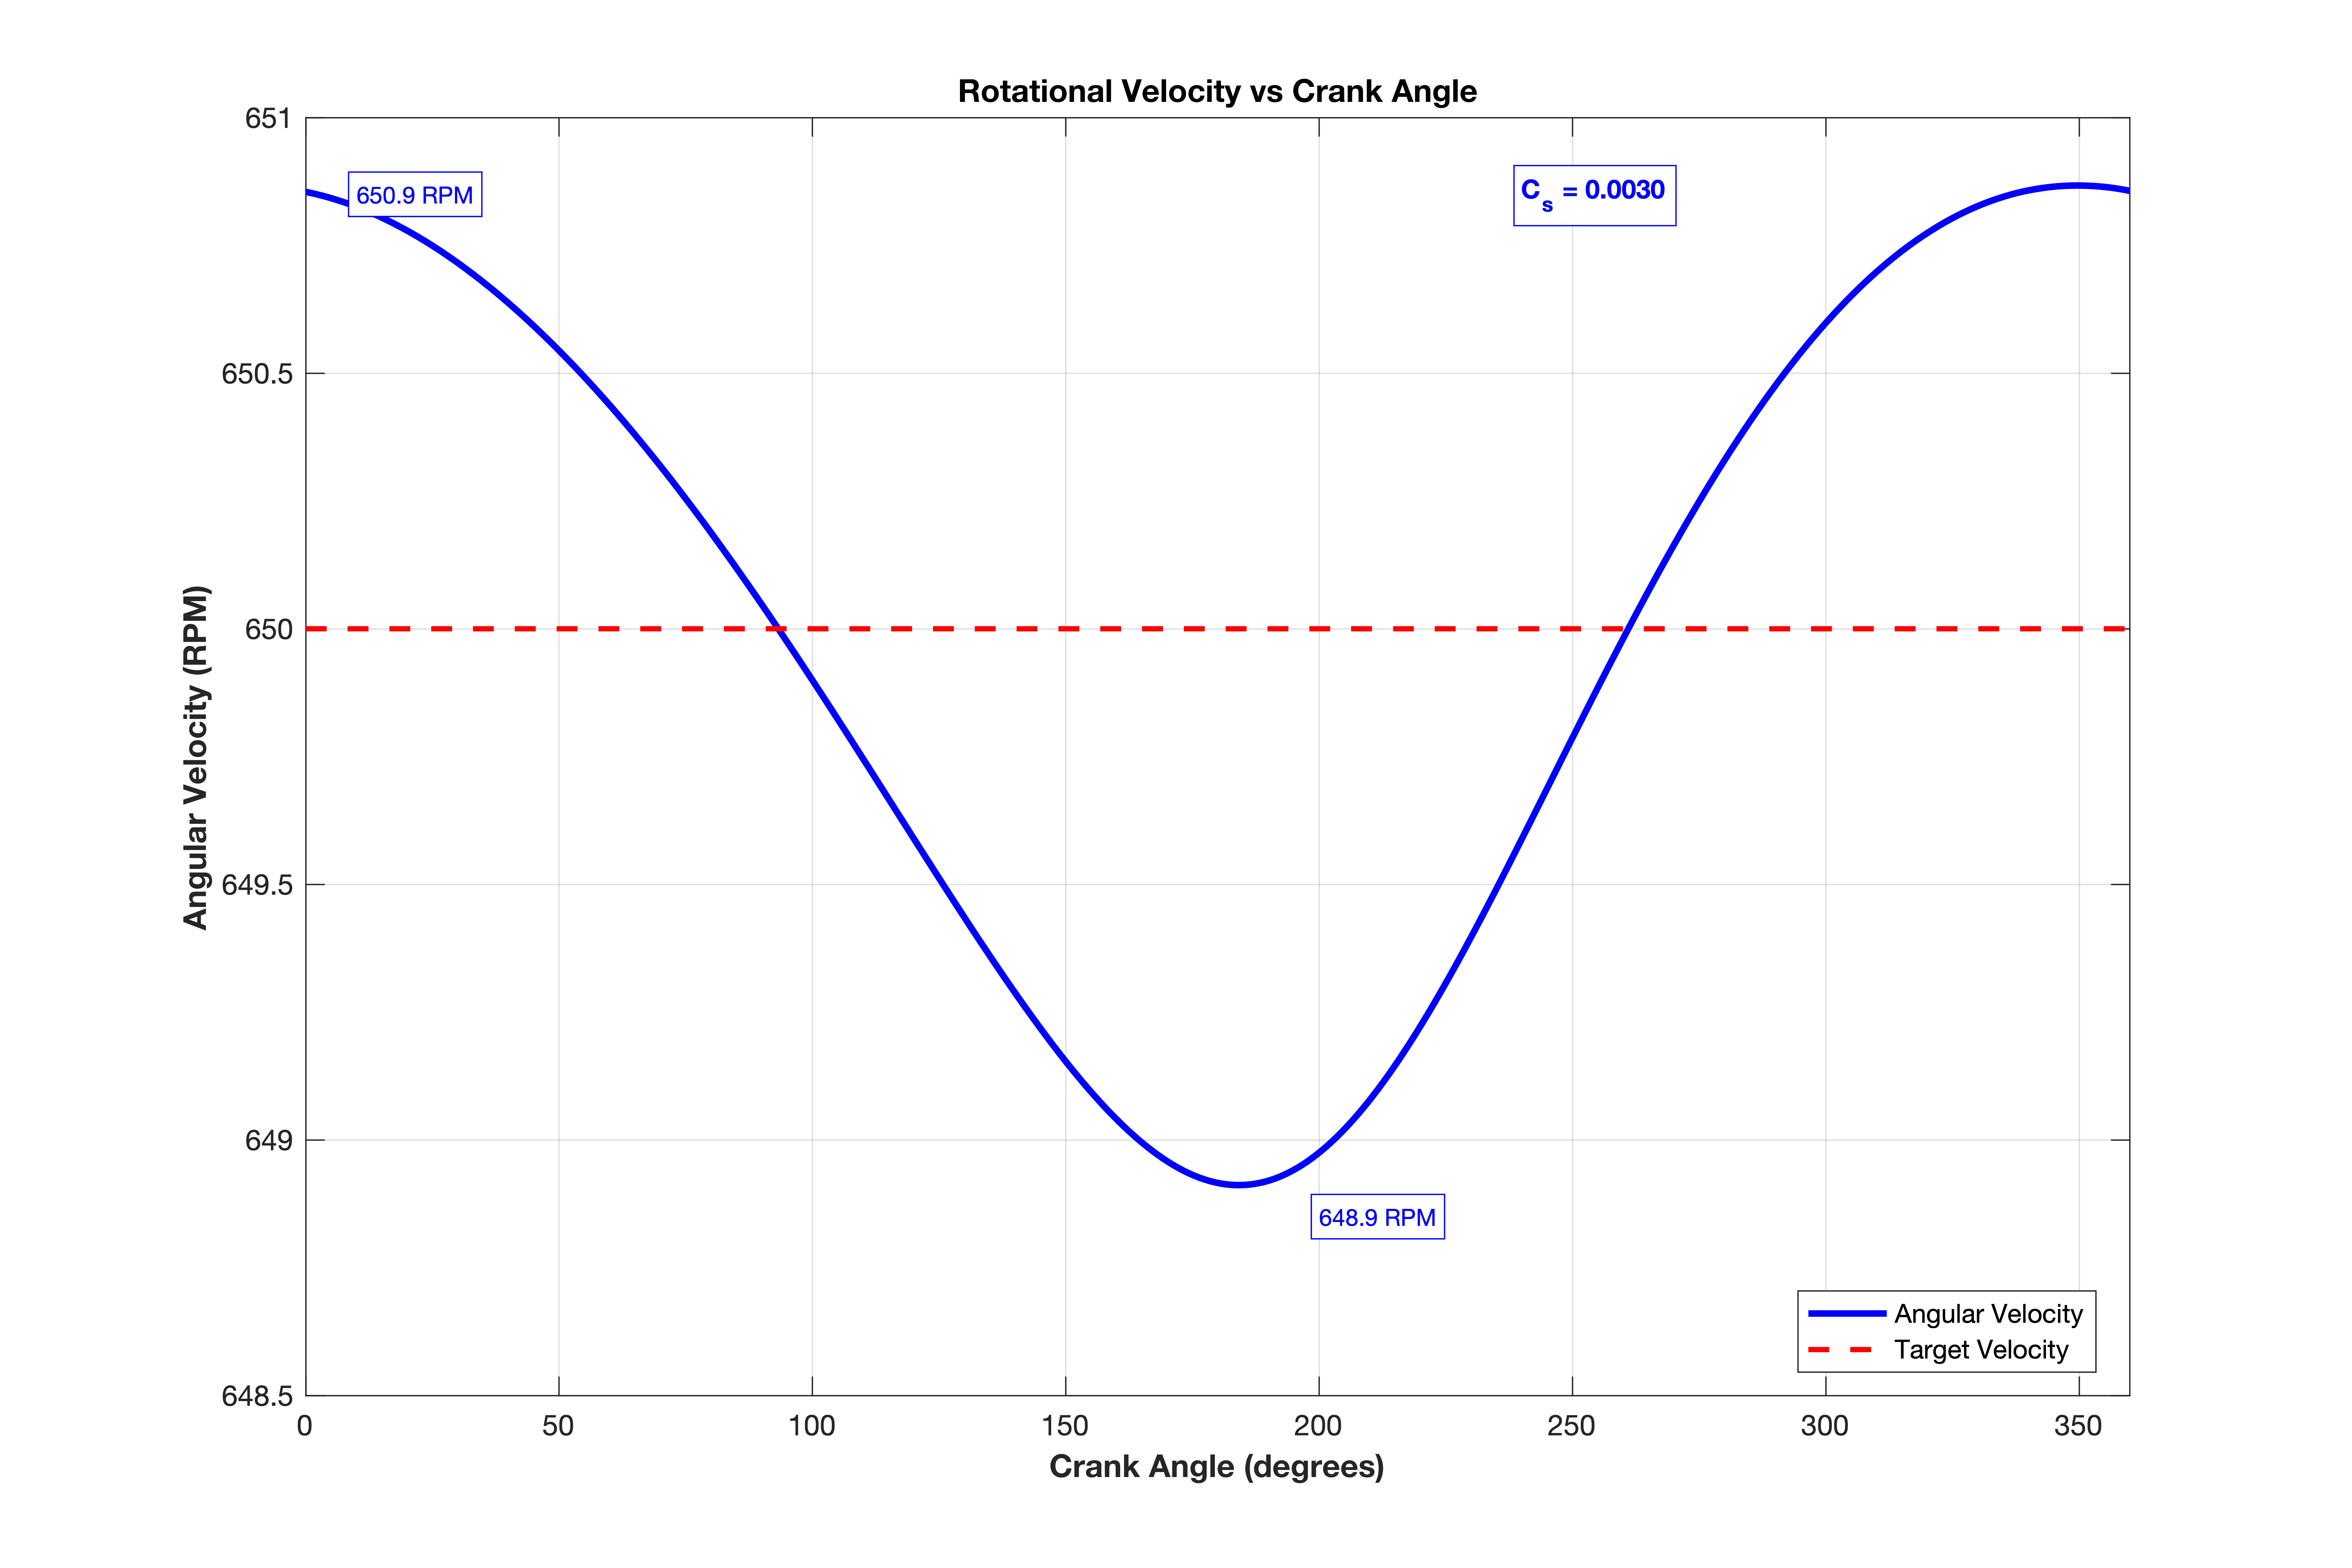
\includegraphics[width=0.8\linewidth]{../angular_velocity.png}
  \caption{Angular velocity vs. crank angle showing the speed regulation achieved by the flywheel.}
  \label{fig:angular_velocity}
\vspace{-6pt}\end{figure}

Operating at 650 RPM target speed, the engine maintains a velocity range of 648.9 to 650.9 RPM, achieving the target coefficient of fluctuation of 0.003. Maximum velocity occurs at 350.0° and minimum at 184.5°, demonstrating effective torque variation smoothing.

The flywheel design requires 4.48 kg·m² moment of inertia, achieved with outer diameter 0.887 m, inner diameter 0.787 m, and mass 25.47 kg. These dimensions are consistent with typical flywheel designs for similar power levels and operating speeds.

\subsection{Phase Optimization}
The phase optimization analysis, shown in Figure~\ref{fig:energy_phase}, reveals the sensitivity of engine performance to phase shift.

\begin{figure}[H]
  \centering
  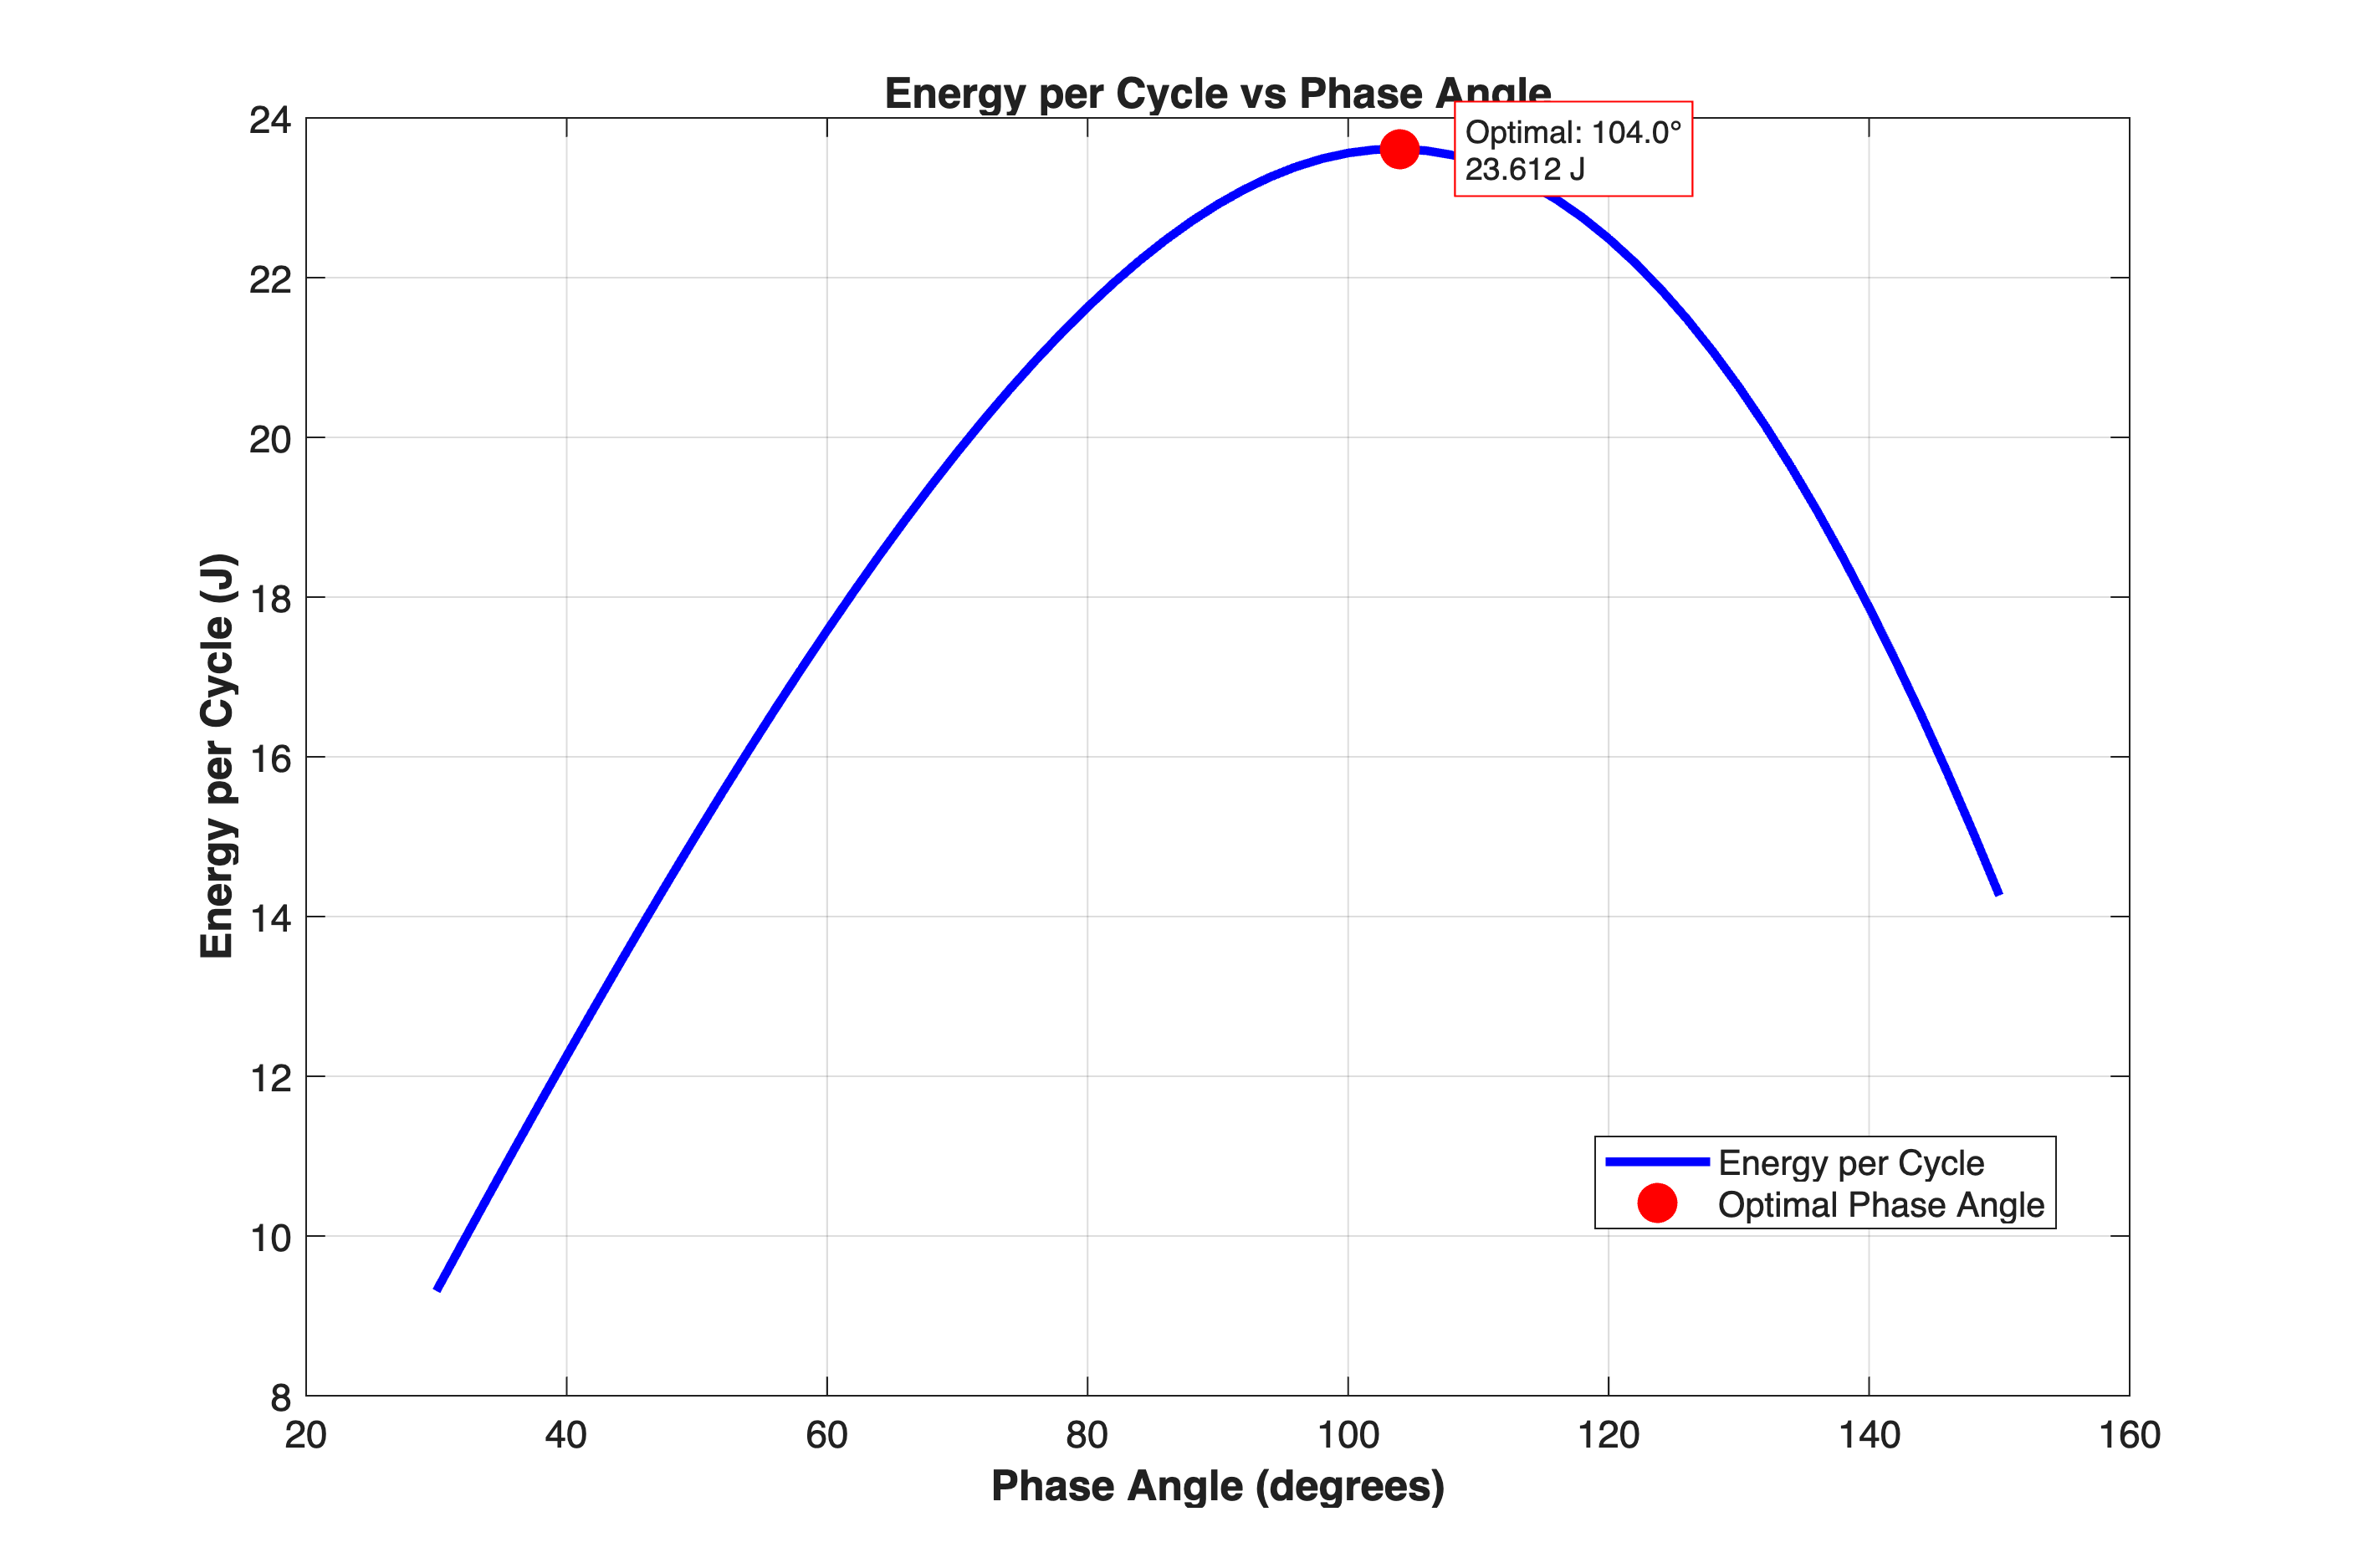
\includegraphics[width=0.8\linewidth]{../energy_vs_phase.png}
  \caption{Energy per cycle vs. phase angle showing the optimization results.}
  \label{fig:energy_phase}
\vspace{-6pt}\end{figure}

The optimization reveals an optimal phase angle of 103.6°, providing maximum power output and representing a 13.6° deviation from the conventional 90° approximation. This significant deviation demonstrates the importance of systematic optimization over simplified assumptions. The three-stage refinement strategy achieves 0.01° resolution for precise optimal point determination.

% (Condensed: key findings and requirement assessment are synthesized in the Conclusion to save space.)

\section{Conclusions and Recommendations}
This analysis successfully demonstrates the complete thermodynamic and dynamic behavior of a Beta-type Stirling engine through systematic computational modeling. The methodology establishes a comprehensive framework where all system variables are expressed as functions of crank angle, enabling parametric studies and design optimization.

\subsection{Thermodynamic Performance}
The pressure-volume analysis reveals significant performance characteristics for the given engine configuration. The ideal Stirling cycle produces 94.9 J of work per cycle, while the actual Schmidt analysis yields 23.0 J, resulting in a cycle efficiency of 24.2\%. This efficiency represents the ratio of actual work output to the theoretical maximum, indicating substantial losses due to non-ideal processes, dead volumes, and the simplified Schmidt assumptions. The positive mean torque of 3.648 N·m confirms the engine's ability to produce net work output over a complete cycle, validating the thermodynamic design.

\subsection{Phase Optimization Results}
Phase shift optimization reveals that the optimal phase angle of 103.6° provides maximum power output, which is 13.6° higher than the conventional 90° approximation. This deviation from the standard value demonstrates the importance of systematic optimization rather than relying on simplified assumptions. The optimization process employed a three-stage refinement strategy, ultimately achieving 0.01° resolution to ensure precise determination of the optimal operating point.

\subsection{Dynamic Behavior and Flywheel Design}
The angular velocity analysis shows excellent speed regulation with minimal fluctuation. Operating at a target speed of 650 RPM, the engine maintains a velocity range of 648.9 to 650.9 RPM, with maximum velocity occurring at 350.0° and minimum velocity at 184.5°. This 2.0 RPM variation corresponds to the target coefficient of fluctuation of 0.003, demonstrating effective flywheel performance.

The flywheel design requirements are substantial but reasonable for the system scale. A moment of inertia of 4.48 kg·m² is required, achieved through a flywheel with an outer diameter of 0.887 m, inner diameter of 0.787 m, and mass of 25.47 kg. These dimensions are consistent with typical flywheel designs for similar power levels and operating speeds.

\subsection{Design Requirements Assessment}
The analysis successfully addresses all specified design requirements. \textbf{Requirements Met:} Flywheel design (4.48 kg·m² moment of inertia, achieving target coefficient of fluctuation of 0.003), power output analysis using two methods (ideal Stirling cycle: 94.9 J/cycle, Schmidt analysis: 23.0 J/cycle), systematic phase optimization identifying optimal angle of 103.6°, and effective speed regulation maintaining 650 RPM ± 1.0 RPM.

\textbf{Performance Limitations:} 24.2\% cycle efficiency indicates significant losses from dead volumes and non-ideal processes. Actual power (23.0 J/cycle) substantially below ideal (94.9 J/cycle) due to Schmidt analysis limitations. Simplified isothermal assumptions overpredict performance compared to real-world conditions.

\end{document}
